\documentclass[11pt]{scrartcl}
\usepackage[a4paper]{geometry}

\usepackage{graphicx}
%\graphicspath{ {./images/} }

\usepackage{fancyhdr}
\pagestyle{fancy}
\fancyhf{}
\fancyhead[L]{ULTRASCHALL - DOPPLER} %Kopfzeile links
\fancyfoot[C]{\thepage}

\usepackage[utf8]{inputenc}
\usepackage{csquotes}
\usepackage[german]{babel}

\usepackage{setspace}

\usepackage{caption}
\usepackage{float}

\usepackage{hyperref}
\usepackage{pdfpages}

\hypersetup{
    pdftitle = {Ultraschall-Doppler},
    pdfsubject = {Biomedizinischesystemtechnik Praktikum},
    pdfauthor = {Leona K{\"o}ck, Chris R{\"u}ttimann},
    pdfkeywords = {} ,
    pdfcreator = {pdflatex},
    pdfproducer = {LaTeX with hyperref}
}

\usepackage[
    style=apa,
    backend=biber,
    sortcites=false,
    sorting=none,
    hyperref=true,
    backref=false
]{biblatex}
\usepackage{amsmath}
\usepackage[T1]{fontenc}
\addbibresource{test.bib}

\setlength{\parindent}{0in}

\begin{document}
    \pagenumbering{Alph}
% ---------------------
% Titlepage
% ---------------------
    \begin{titlepage}
        \begin{center}
        {\LARGE OST Ostschweizer Fachhochschule}
            \\[1.5cm]
            \linespread{1.2}\large { Biomedizinischesystemtechnik Praktikum }

            \huge{\bfseries Ultraschall-Doppler}
            \\%[1.5cm]
            \large{durchgef{\"u}hrt am 22. März 2021}
            \\[1.5cm]
   %         \linespread{1}
           
\includegraphics[width=8cm]{../images/ost_logo.eps}
           \\[1cm]
            {\small{Autoren}}\\
            {\Large{Leona K{\"o}ck}}\\
            {\Large{Chris R{\"u}ttimann}}
            \\[1cm]

            \vspace*{\fill}
            \large{\today}
        \end{center}

    \end{titlepage}

% ---------------------
% Abstract
% ---------------------
    \pagenumbering{Roman}
 %   \pdfbookmark[section]{Abstract}{abstract}
 %   \section*{Abstract}
    \addtocounter{section}{0}

 %   \pagebreak
    \setstretch{1.25}
% ---------------------
% Table of contents
% ---------------------
    \tableofcontents
    \pagebreak


% ---------------------
% Body
% ---------------------
    \pagenumbering{arabic}

    \section{Problem- und Zielvorstellung}
    Ziel dieses Praktikums war es, die Vorteile der nichtinvasiven Messmethode nach dem Prinzip \emph{Continuous Wave Doppler}
    kennenzulernen sowie die bereits vorhandenen Kenntnisse aus der Vorlesung mit praktischen Versuchen zu vertiefen.
    \section{Problemlösung}
    \subsection{Vorbereitung}
   Das Praktikum wurde anhand der Angaben aus \cite{Doppler} durchgeführt.
    
    Für der Versuch wurden folgende Materialien benötigt:
    \begin{itemize}
        \item Dopplergerät HiDop 360 
        \item PC mit der Software HiDop
        \item 4MHz und 8MHz Transducer
        \item 4MHz Test-Transducer 
        \item Halterung für zwei Transducer
        \item Funktionsgenerator HMF 2550 
        \item Gel
    \end{itemize}


    \subsection{Messung}
    \subsubsection{HiDop 360}
    Die erste Aufgabe bestand darin, sich mit dem Dopler-Messgerät vertraut zu machen 
    und dessen wichtigsten Funktionen kennen zu lernen.
    Dazu gehörte unter anderem die zwei Sonden mit dem Messgerät zu verbinden, das Messgerät
    wiederum mit dem PC zu verbinden sowie das Programm HiDop zu starten.
    Es wurde ein Patient angelegt um die folgenden Messungen speichern zu können.
    %todo Eventuell Messaufbau zeichnen? nöö

    \subsubsection{Ausmessen des Dopplergerätes HiDop 360}
    Die zweite Aufgabe war es, mithilfe eines Sonogramms zu überprüfen, ob das Dopplergerät funktioniert und richtig geeicht ist. 
    Dazu wurde der der 4MHz Transducer des Messgeräts sowie der Testtranducer in die Halterung mit ca. einem Millimeter Abstand eingespannt.
    Um eine gute Übertragung des Signals zu gewährleisten, wurde der Zwischenraum mit Ultraschall-Gel gefüllt.
    Der Testtranducer war mithilfe eines Abschwächers an den Funktionsgenerator, der ein 4.001MHz Sinussignal liefert, angeschlossen. 
    Die Verbindung mit dem PC wurde genutzt, um das Sonogramm besser darzustellen und speichern zu könnnen.
    Am Gerät selbst wurde der 5kHz Messbereich, eine Zeitablenkung von 4s sowie die Sonogrammdarstellung gewählt.

    \subsubsection{Testmessung an Gefässen}
    Um Messungen an den Gefässen der Probanden vorzunehmen wurde auf den 8MHz Transducer gewechselt. 
    Am Dopplergerät wurdend die Dopplerindizies S/D und RI eingestellt.
    Bei den beiden Probanden Chris Rüttimann und Leona Köck wurden die Messungen sowohl an der Carotis Communis
    (Halsschalgader), als auch an der Arteria Radialis (Handgelenk) durchgeführt.

    \section{Ergebnisse}
    \subsubsection{Ausmessen des Dopplergerätes HiDop 360}
    Wie nach lesen der Aufgabe zu erwarten war, stimmte die gemessene Frequenz des Dopplergeräts nicht genau mit der des Funtionsgenerators überein.
    Zu sehen ist dies in der \autoref{fig:offset}.
    Das ist der Fall, weil der Funktionsgenerator genauer ist als das medizinische Messgerät.
    Die Frequenz des Quarzes des Dopplergerätes weicht aufgrund von Temperatur und Alter ab, welches normal ist.
    Diese Differenz wird in ppm angegeben, wobei 100ppm bei medizinischen Messgeräten dem Standard entspricht.
    Berechnet man dies, würde das für diese Messung schon eine Differenz von 400Hz bedeuten. 
    Die Abweichung ist bei dem Messgerät nicht von grosser Bedeutung, da durch den verwendeten Demodulator lediglich
    das Differenzsignal (=Dopplerfrequenz, 1kHz) erhalten bleibt.\\
    Um die angestrebten 4.001MHz zu erreichen wurden das Signal des Funktionsgenerators um 180Hz erhöht.

    \begin{figure}[H]
        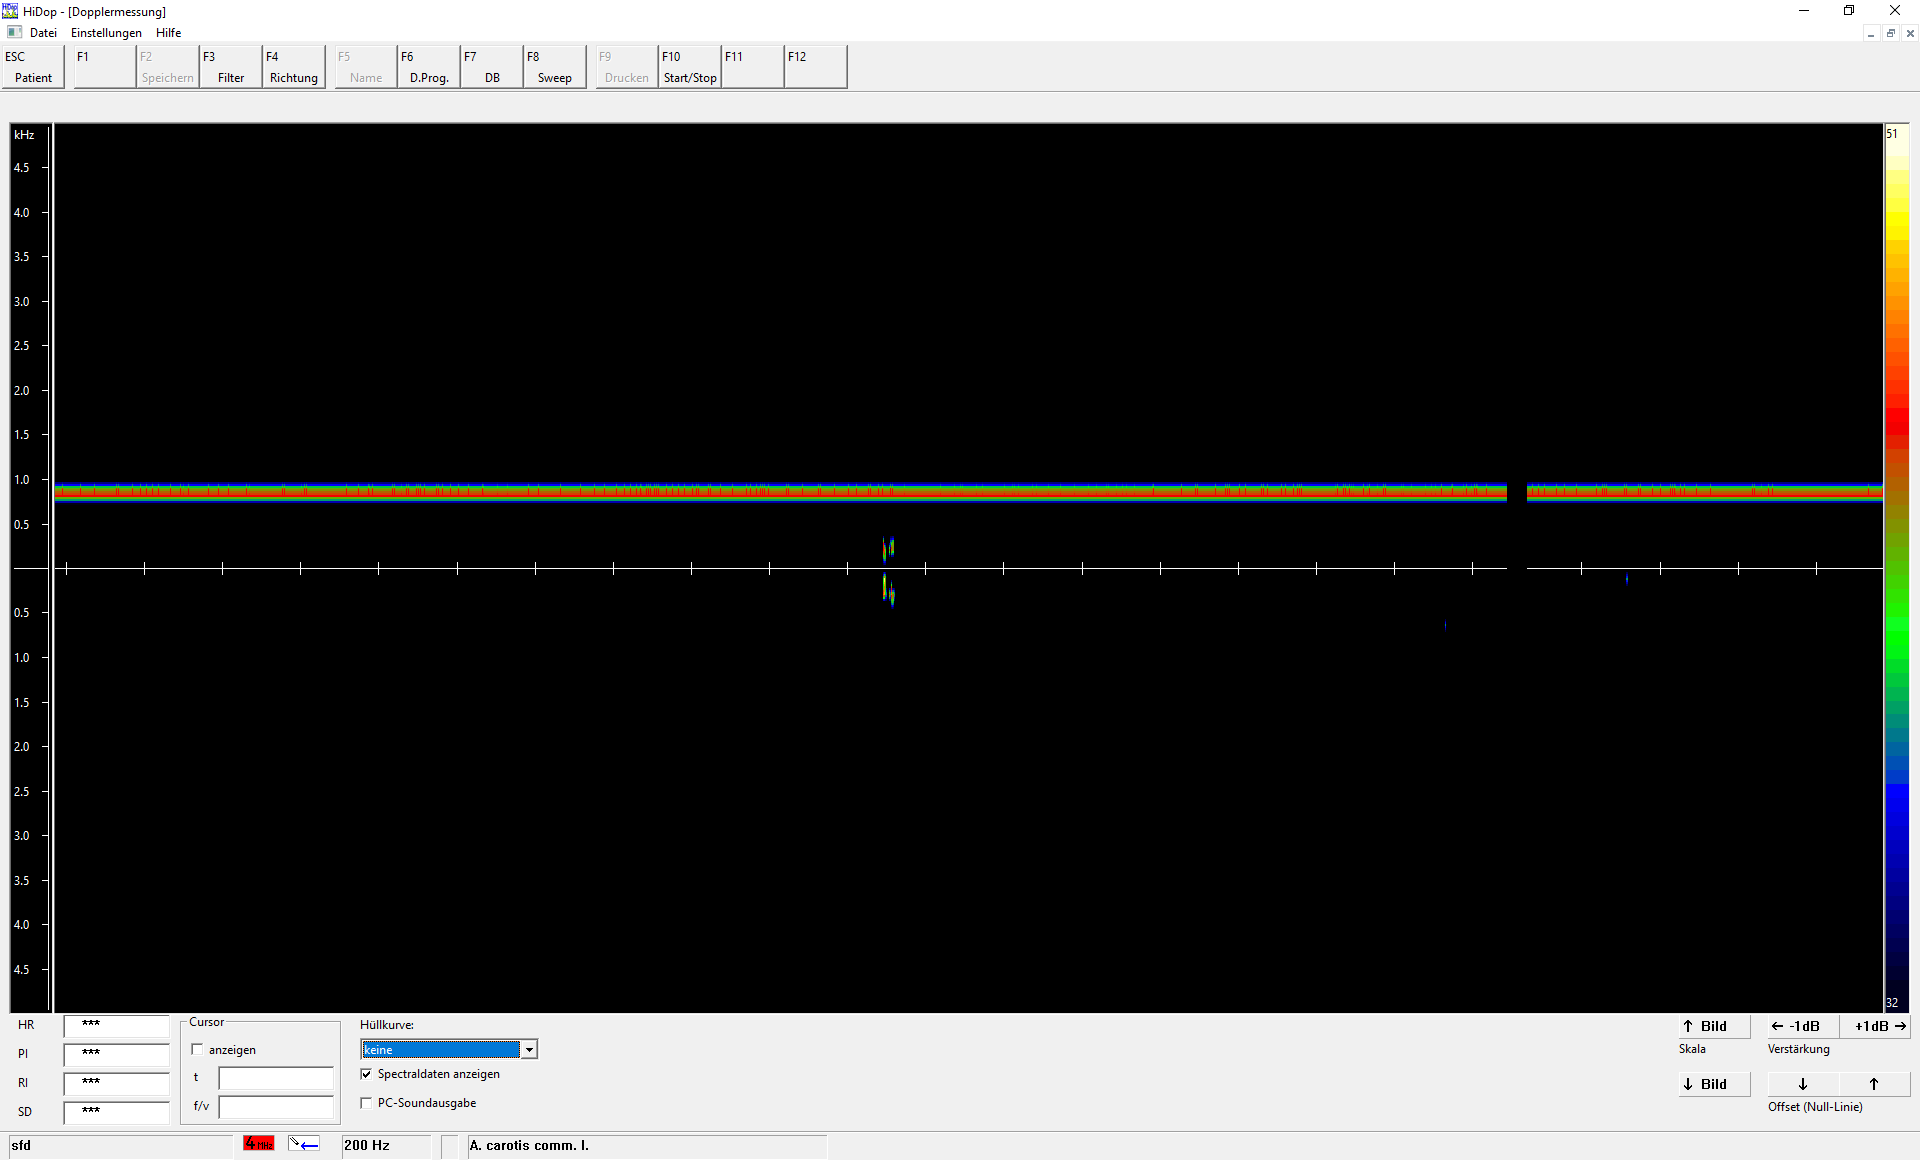
\includegraphics[width=16cm]{images/4001MHz.png}
        \caption{Offset Dopplergerät, eigene Grafik}
        \label{fig:offset}
    \end{figure}

    \subsubsection{Testmessung an Gefässen}
    Bei der Messung selbst ist die gemessene Frequenz kaum von Bedeutung, das Hauptaugenmerk liegt auf dem Muster.
    Dieses Muster ist sehr komplex und variiert stark nach Messstelle.
    Nur erfahrene Ärzte können dieses Muster zuverlässig interpretieren.

    Die Untersuchung der Halsschlagader mit Ultraschall wird in den meisten Fällen zur Kontrolle oder Diagnostizierung
    einer Verengung, einer sogennanten Karotisstenose, durchgeführt.
    Dadurch könnten präventive Massnahmen gegen einen Schlaganfall eingeleitet werden.

    Beim Proband Rüttimann war es sowohl am Hals auch am Handgelenk sehr einfach ein passendes Signal zu erhalten.

    Bei Frau Köck war es leider nicht so einfach ein durchgehendes Signal an der Halsschlagader zu erhalten.
    Schliesslich konnte nach Einhaltung des 60° Winkels des Transducers am Vorderrand gemessen werden.

    Gemäss \cite{duplex} sollte das Muster zwischen Handgelenk und Hals eindeutig unterscheidbar sein.
    Vor allem bei der Halsschlagader ist das Messergebnis schwierig zu deuten, da sich die Stelle der Messung in etwa
    der Karotisgabel (Bifurcation carotidis) befindet.
    Dort teilt sich die Arteria Carota Communis (ACC) in zwei Gefässe: die Arteria carotis interna (ACI) und die
    Arteria carotis externa (ACE).
    Alle diese Gefässe unterscheiden sich in ihrem Flussbild.
    Bei Frau Köck könnte es sich um die ACE handeln, da ein leichtes triphasische Flussprofil vorhanden ist.
    Herr Rüttimann hat vermutlich die ACI aufgenommen.
    Ohne hinreichende Erfahrung lässt sich nicht genau sagen, welche Arterie gemessen wurde.
    Leider sind (Normal-)Befunde für die Aretria Radialis schwer zu finden.
    Daher kann an dieser Stelle keine Aussage über diese Messungen getroffen werden.
    %Die Messungen an den zwei Probanden zeigen auch unterschiedliche Muster, jedoch zeigt die Handmessung das
    %Halsmuster und umgekehrt.
    %Vermutlich ist bei der Beschriftung der Messungen ein Fehler unterlaufen, dies ist jetzt jedoch nicht mehr
    %nachvollziehbar.

    % Es ist sehr auffallend, dass bei
    %done: https://www.unispital-basel.ch/fileadmin/unispitalbaselch/Departemente/DKTT/Angiologie/Fortbildungen
    %/Duplexsonografie19/DE/1.2_Spektralanalyse_Pr%c3%a4sentation_DE_2019.pdf
    % eigentlich: zwei zacken voll klar erkennbar, druck im hals größer als an der hand
    % stimmt aber eig nicht weil bei chris stimmt iwie ned?
    % https://books.google.at/books?id=dXOdMycV-ywC&pg=PA20&lpg=PA20&dq=Frequenzspektrumanalyse+(Spektral-Doppler-Modus)&source=bl&ots=ZvsKNNZHkN&sig=ACfU3U0fP4vO176HsbUE-54bNMch6Dv2SQ&hl=de&sa=X&ved=2ahUKEwjVw_bNrdbwAhWC3KQKHVYxATAQ6AEwD3oECBAQAw#v=onepage&q=Frequenzspektrumanalyse%20(Spektral-Doppler-Modus)&f=false
    % sieht aber gut aus, keine schlimmen anzeichen für stenose

    %Frequenz nicht so wichtig .... Muster ist wichtiger ... ist aber bei jeder Stelle anderst und andere
    %Ausprägungen bedeuten andere Sachen -> sehr komplex
    %Messwinkel ca. 60 Grad beachten (in Flussrichtung)
    %... Bewegungsartefakte vermeiden
    %messungen am liegenden Patient würden bessere ERgebnisse erzielen
    % deutung: https://www.kup.at/kup/pdf/3947.pdf sieht vielversprechend aus... weiß aber nicht ob wir das brauchen, wird nicht erwartet ... 

     %Chris: sehr leicht
     %Leona: schwer zu finden.... auf Ton hören hilft

    \begin{figure}[H]
        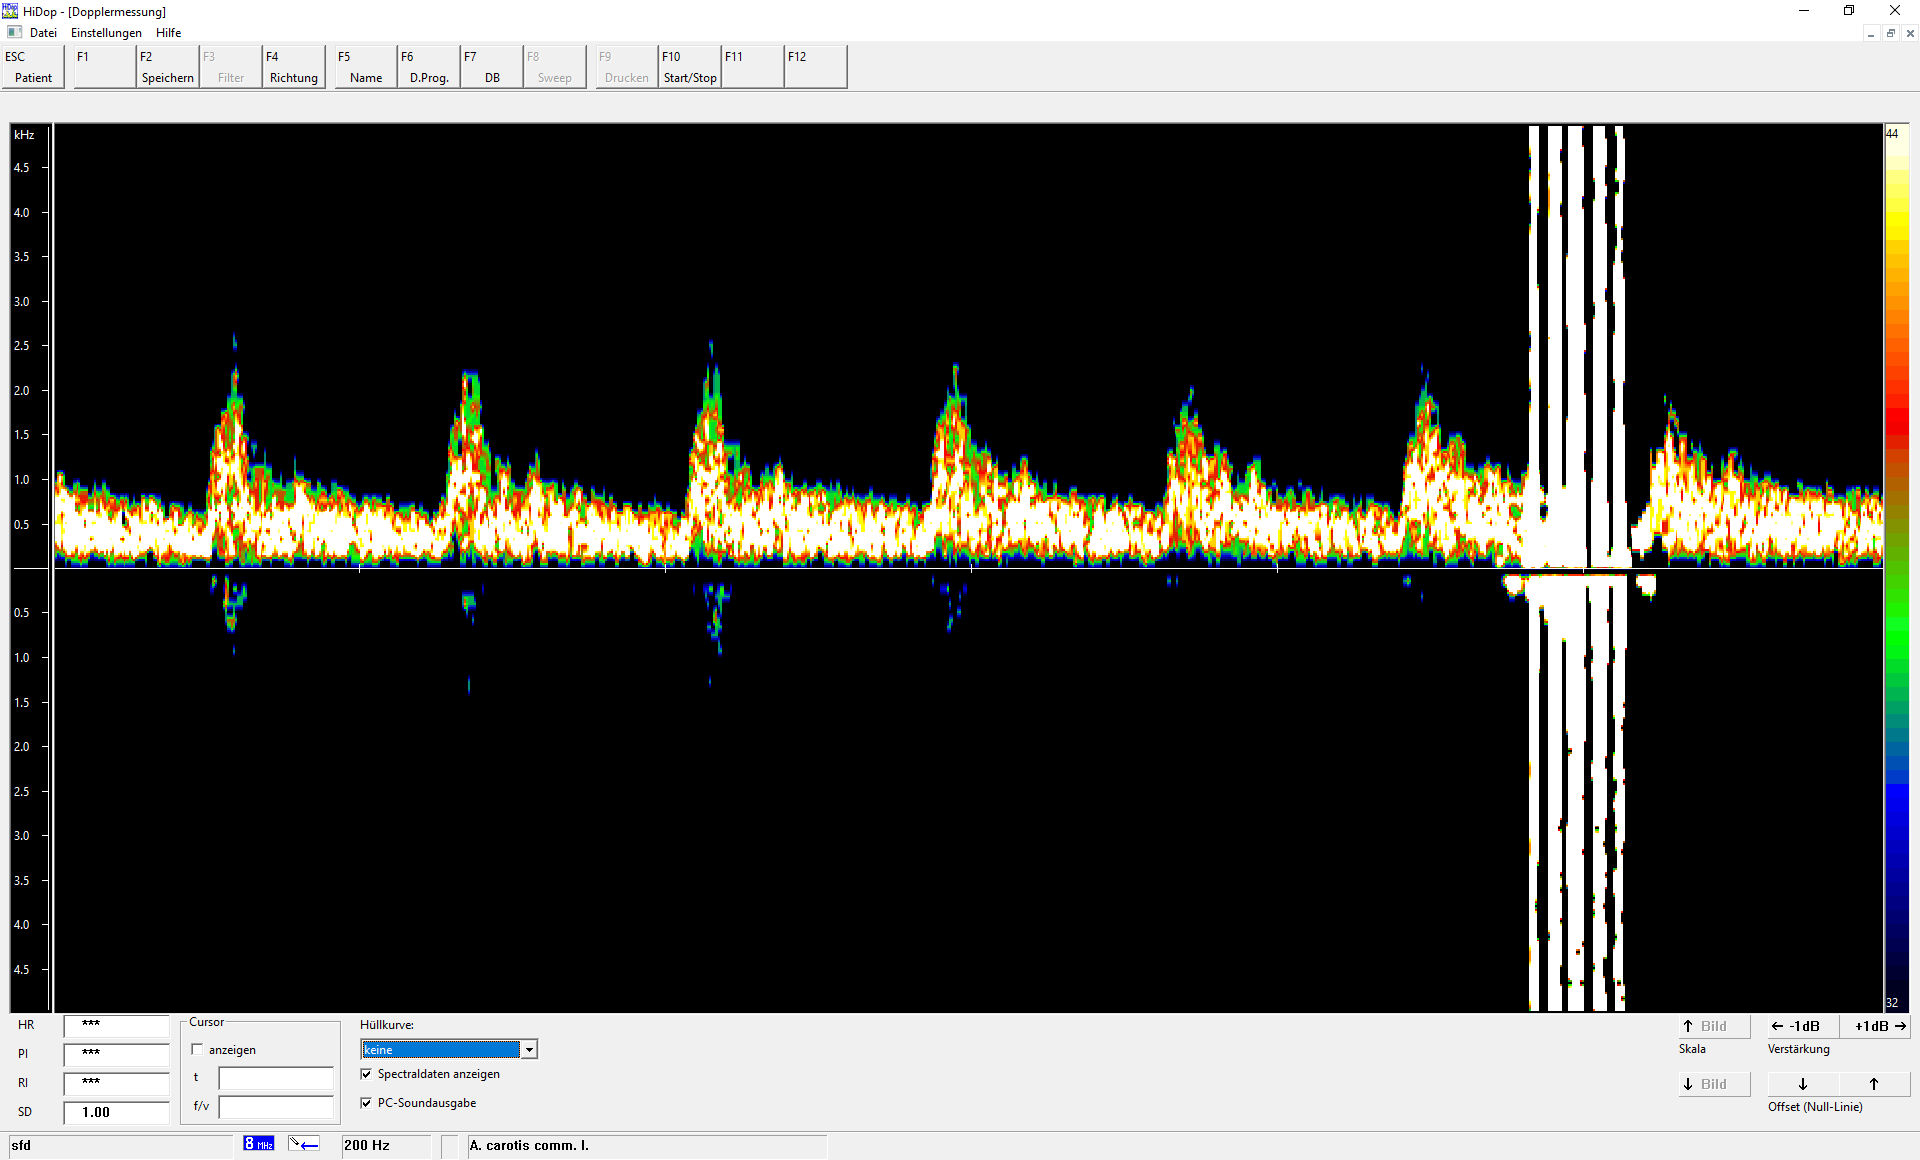
\includegraphics[width=15cm]{images/Chris_Hals.png}
        \caption{Rüttimann Halsschlagader, eigene Grafik}
    \end{figure}
    \begin{figure}[H]
        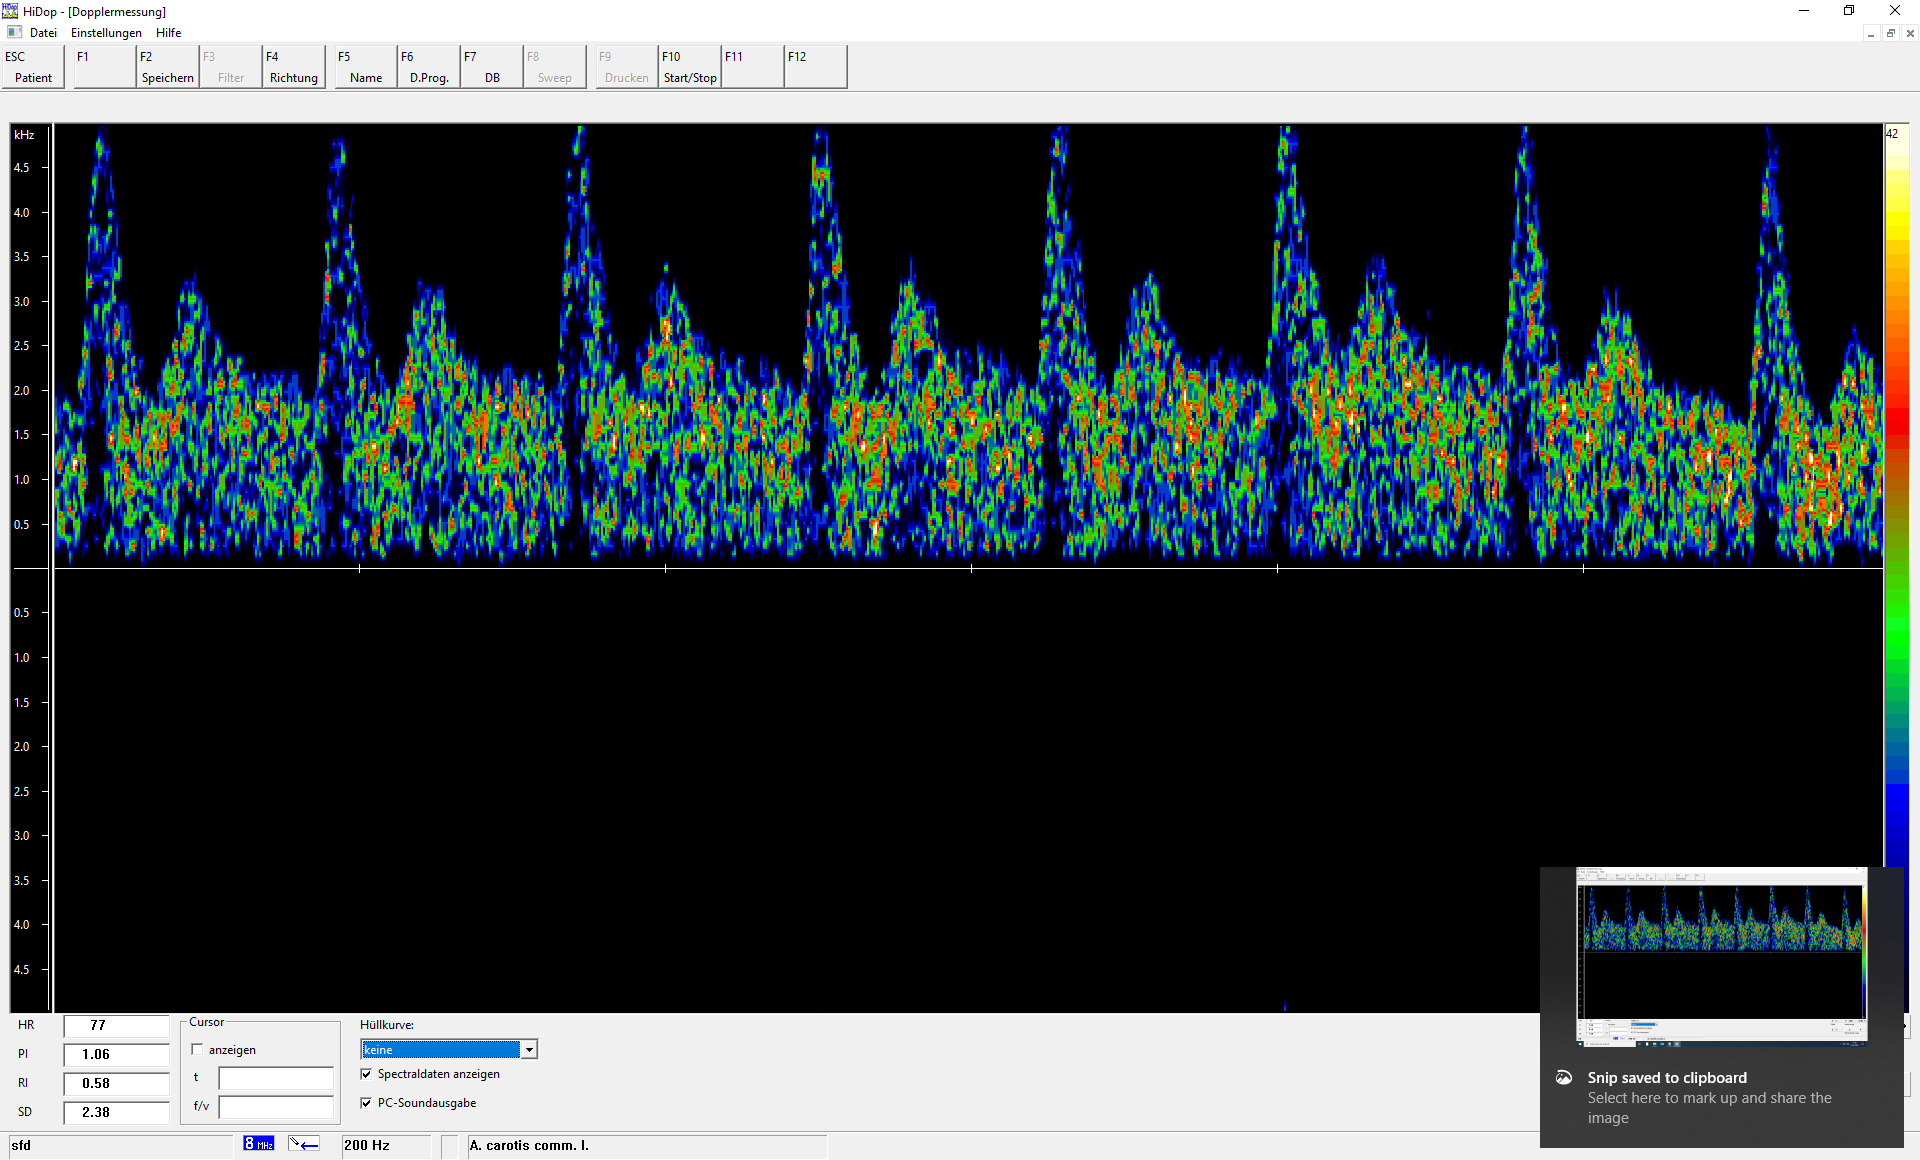
\includegraphics[width=15cm]{images/Chris_Handgelenk.png}
        \caption{Rüttimann Handgelenk, eigene Grafik}
    \end{figure}
    \begin{figure}[H]
        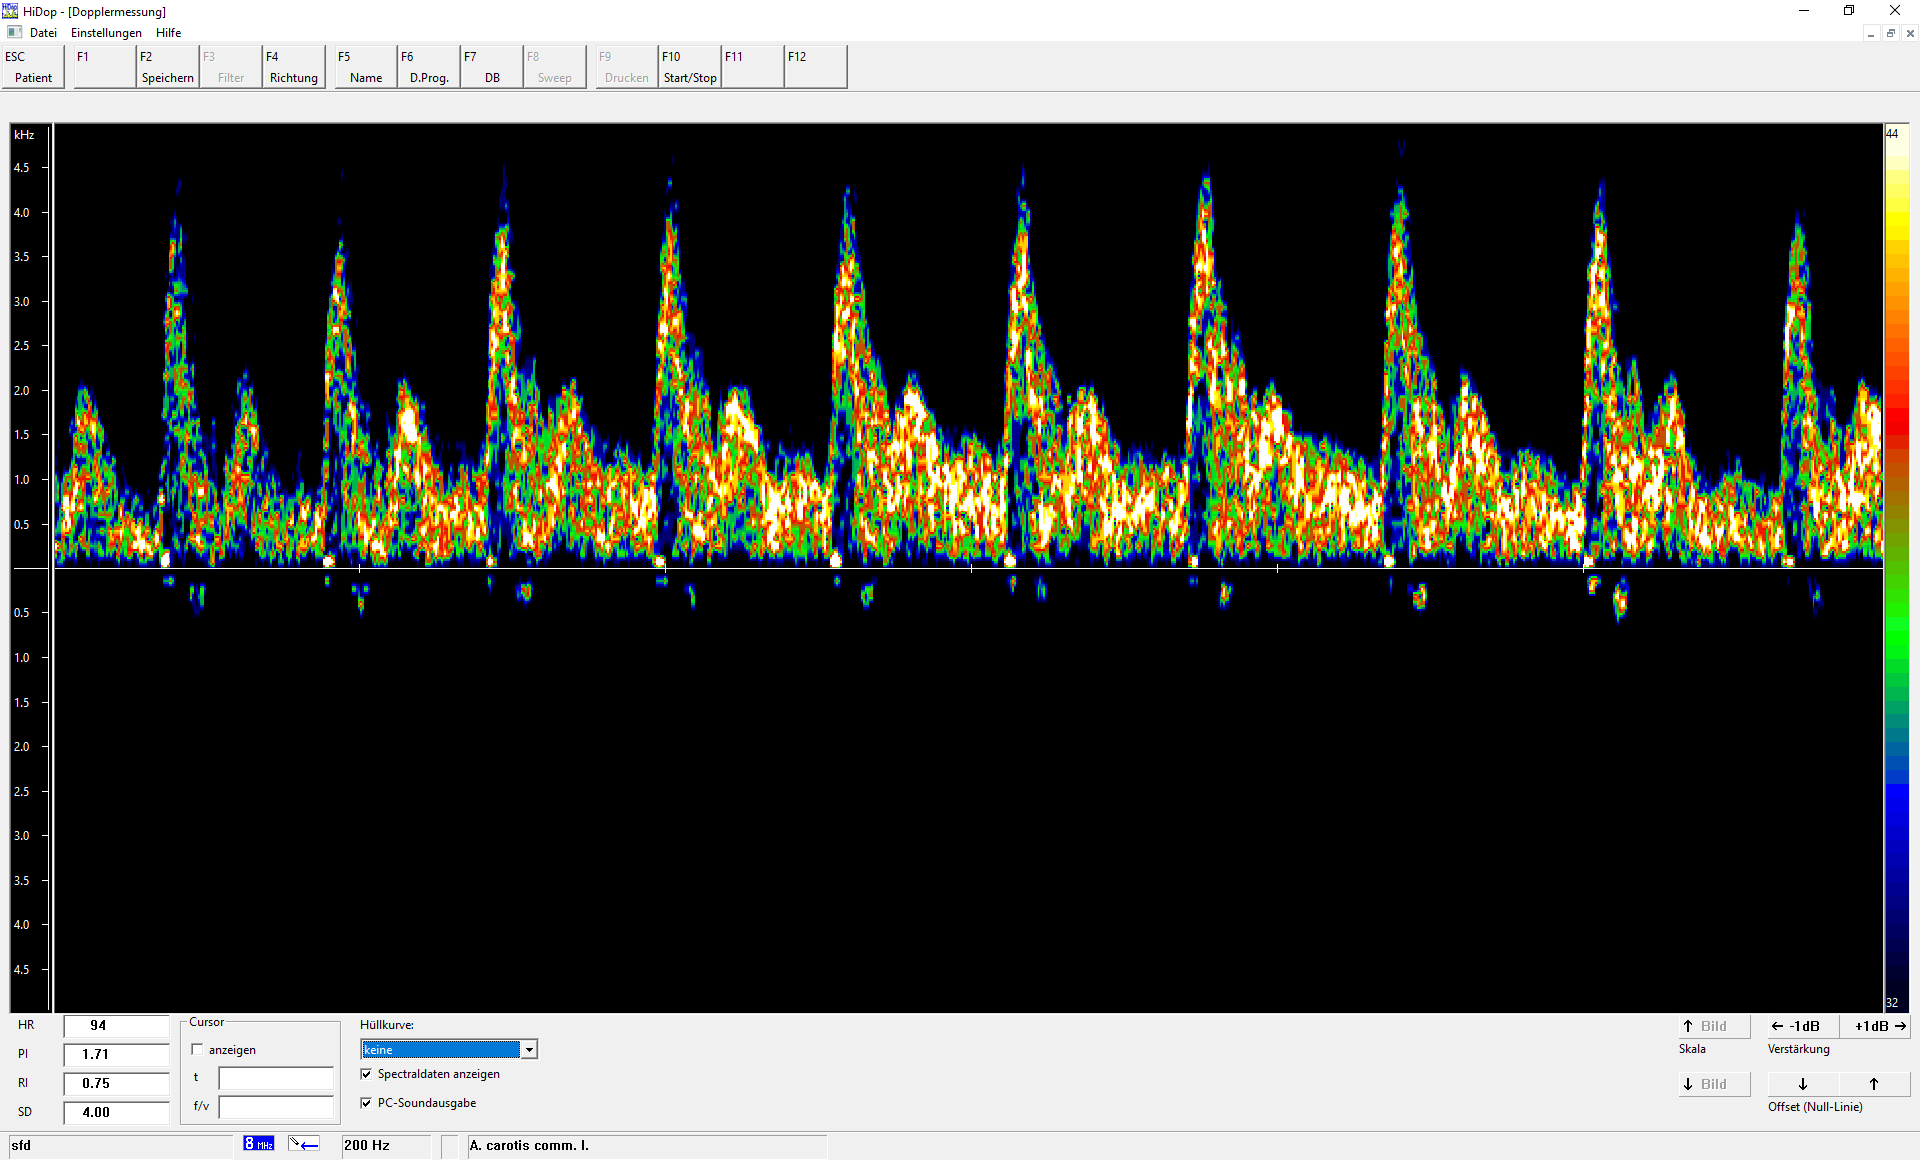
\includegraphics[width=15cm]{images/Leona_Hals.png}
        \caption{Köck Halsschlagader, eigene Grafik}
    \end{figure}
    \begin{figure}[H]
        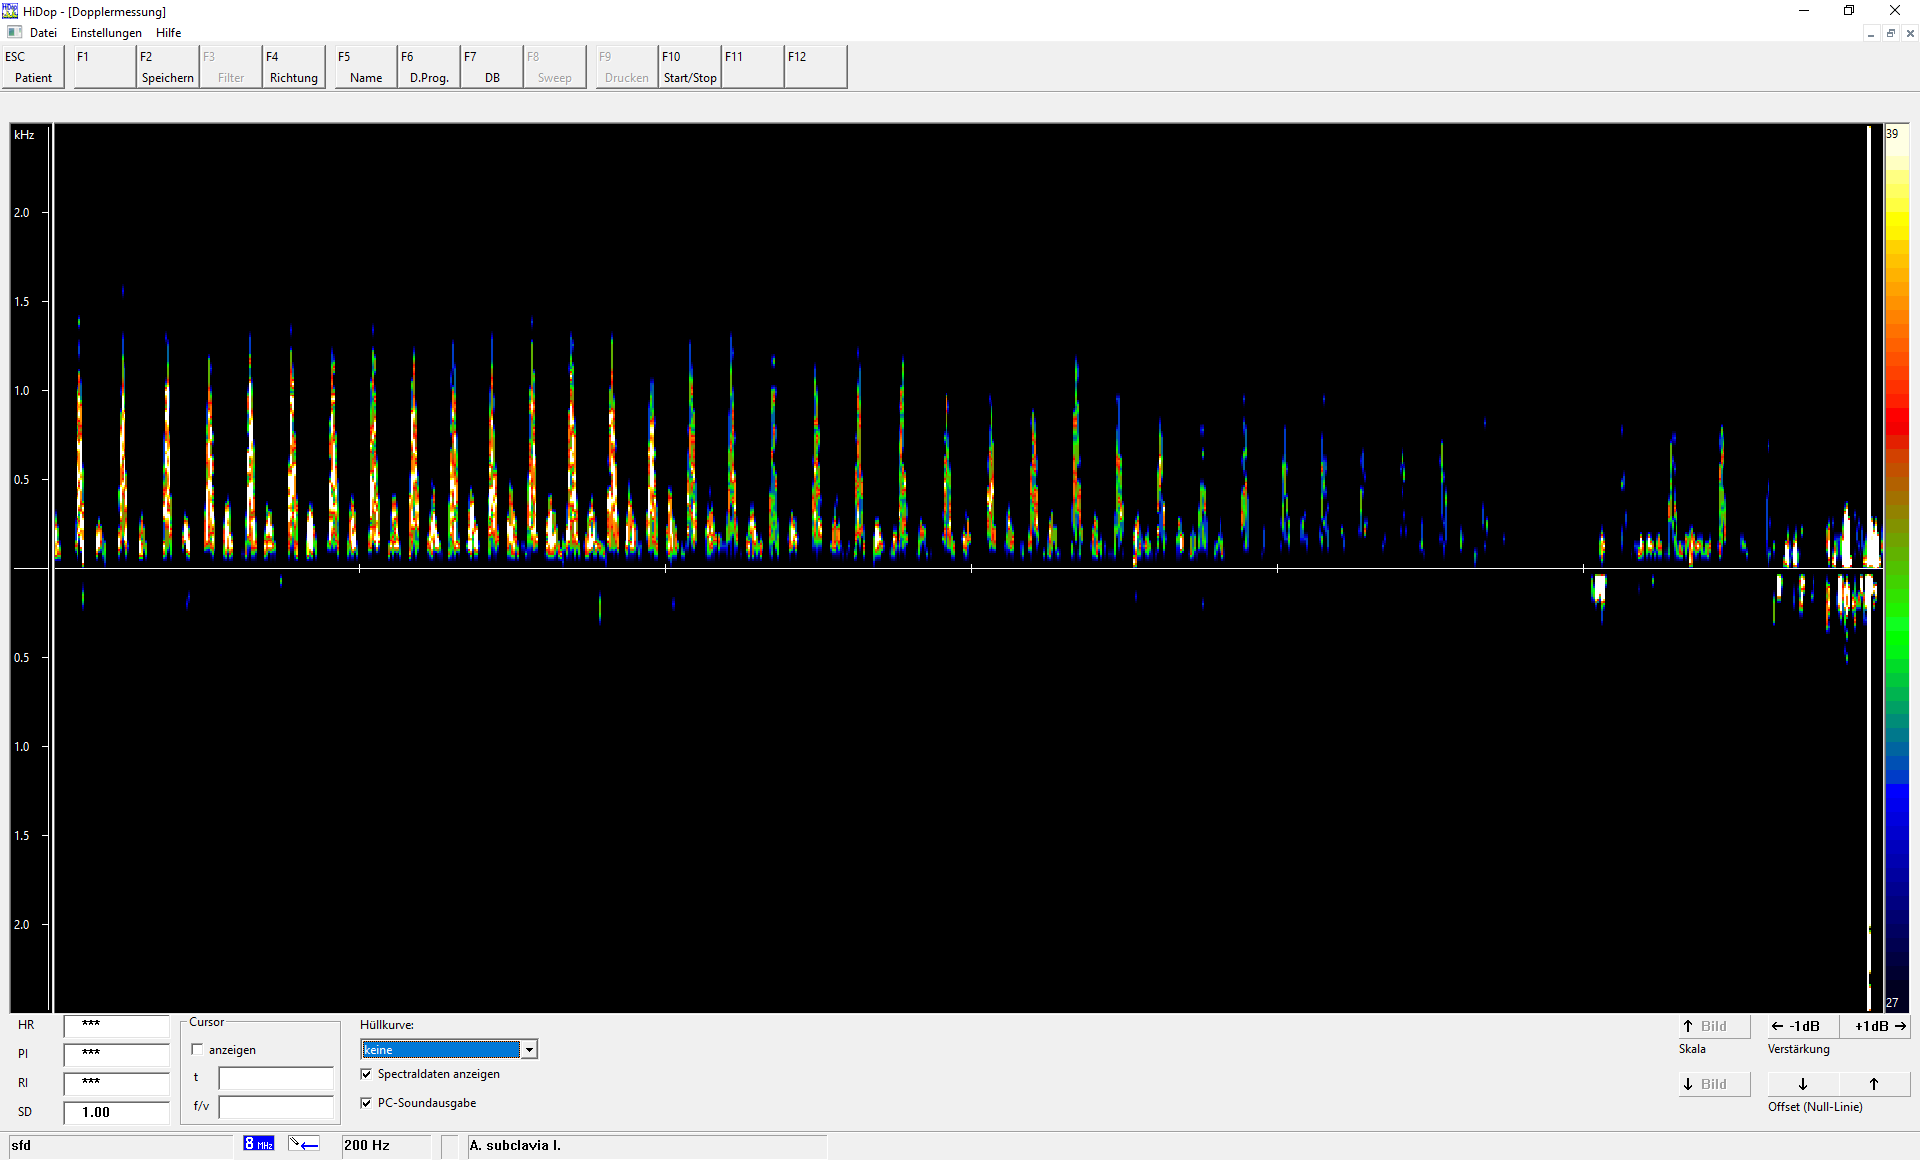
\includegraphics[width=15cm]{images/Leona_Handgelenk.png}
        \caption{Köck Handgelenk, eigene Grafik}
    \end{figure}

    \pagebreak

    \subsubsection{FFT}

    \autoref{fig:fft} zeigt einen Screenshot des zweiseitige logarithmische Power-Spektrums.
    Dies wurde mit den Daten aus HiDopData und dem zur Verfügung gestelltem Matlab Skript erstellt.
    Jedes Gefäss erzeugt ein für sich eindeutiges Spektrum, welches durch eine Fachperson auf mögliche Defekte interpretiert werden kann.

    \begin{figure}[H]
        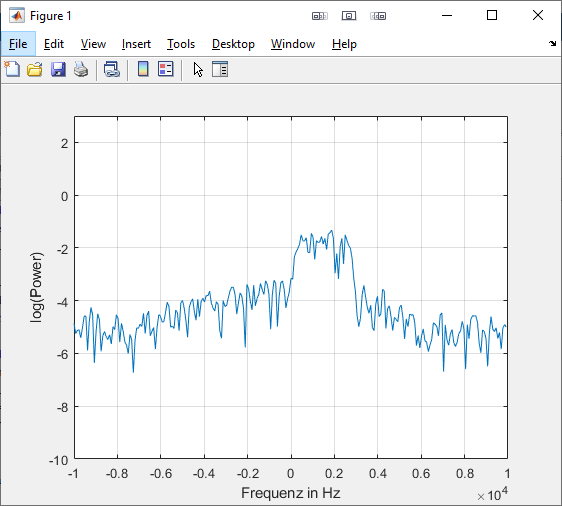
\includegraphics[width=16cm]{images/Movie_Screenshot}
        \caption{Screenshot Power-Spektrum, eigene Grafik}
        \label{fig:fft}
    \end{figure}

    \pagebreak

    \section*{Eigenständigkeitserklärung}
    \addcontentsline{toc}{section}{Eigenständigkeitserklärung}

    Hiermit bestätigen wir, dass wir diesen Bericht selbstständig und ohne fremde Hilfe verfasst haben.
    Alle verwendeten Quellen wurden entsprechend dem APA-Standard gekennzeichnet.
    \\[3cm]


    \begin{figure}[H]
        
\includegraphics[width=4cm]{.././images/Unterschrift_Leona.png}
    \end{figure}
    \begin{tabular}{@{} l@{}}
        \hline \\
        \makebox[6cm]{Leona Köck}\\[2cm]
    \end{tabular}


    \begin{figure}[H]
        
\includegraphics[width=4cm]{.././images/Unterschrift_Chris.png}
    \end{figure}
    \begin{tabular}{@{} l@{}}
        \hline\\
        \makebox[6cm]{Chris Rüttimann}
    \end{tabular}

    \pagebreak
% ---------------------
% References
% ---------------------
    %\printbibliography
    \addcontentsline{toc}{section}{Literaturverzeichnis}

% ---------------------
% List of figures
% ---------------------
%    \listoffigures
%    \addcontentsline{toc}{section}{Abbildungsverzeichnis}
%    \pagebreak

% ---------------------
% List of tables
% ---------------------
%\listoftables



% ---------------------
% Anhang
% ---------------------
%\appendix

\end{document}